%\setcounter{section}{6}
\section{ЭЛЕМЕНТЫ ДИНАМИЧЕСКОГО ПРОГРАММИРОВАНИЯ}
\indentПод динамическим программированием понимается метод оптимизации для операций, которые можно разбить на ряд шагов (этапов). Выбор решений на отдельных этапах можно рассматривать как управление реализацией данной операции. Для точной постановки задачи требуется введение некоторых новых понятий.

\subsection{ Прикладной пример и основные понятия}

\indentНа ферме имеется стадо скота. Ежегодно часть стада отправляется на мясозаготовки, а остальная часть остается на ферме для воспроизводства. Доход от продажи скота выражается функцией $\varphi$(u), где u — количество  проданного  скота. Функция $\varphi$(u) может иметь, например, следующий вид Рис. \ref{picture_7_1}

\begin{figure}[h]
\center{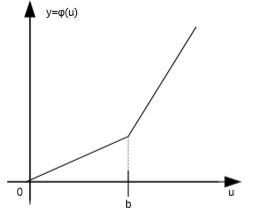
\includegraphics[scale=1]{pictures/picturefile_7_1}}
\caption{Зависимость цены от количества проданного скота}
\label{picture_7_1}
\end{figure}

 Здесь поставки мяса сверх планового задания $\it b$ оплачиваются по  более высокой цене. Количество скота, оставленного на ферме для воспроизводства, в следующем году до начала мясозаготовок увеличивается в $\it a$ раз, где $\it a$ $\ge$1. Требуется таким образом спланировать мясозаготовки на $\it N$ лет, чтобы в итоге пoлучить максимальный доход при условии, что минимальные ежегодные мясозаготовки составляют $\it b$ .
\newpage
Обозначим через $\it x$(0) начальное количество скота на ферме, а через $\it x(t)$ — количество скота, оставленного на ферме к концу$\it t$-го года,$\it t=1,2,...,N$.\\
\indentКоличество голов скота, проданного для мясозаготовок в $\it t$-м году, обозначим через $\it u(t), t=1,2,...,N$. В $\it t-1$ году, было оставлено для воспроизводства количество скота, равное $\it x(t-1)$. Следовательно, в $\it t$-м году перед мясозаготовками количество скота будет $\it ax(t-1)$. Из этого количества $\it u(t)$ будет продано для мясозаготовок, а остальная часть, т.е. $\it ax(t-1)-u(t)$, останется на ферме для воспроизводства. Доход фермы за $\it N $лет составит:\numberwithin{equation}{section}\begin{equation*}
I=\varphi(u(1)) + \varphi(u(2)) + \varphi(u(N))=\sum_{t=1}^N \varphi(u(t))\end{equation*}
\indentУчитывая обязательные мясозаготовки, мы имеем для управляющего параметра $\it {u(t)}$ ограничения :\numberwithin{equation}
{section}\begin{equation*} {u(t) \ge b,   t=1,2,...,N.} \end{equation*}
\indentКроме того, естественно считать выполненным условие \numberwithin{equation}
 {section}\begin{equation*} x(N)\ge d , \end{equation*}
где $\it d$ — плановое задание по разведению скота к концу $\it N$-летнего периода.\\
\indentИтак, мы можем сформулировать следующую математическую задачу: требуется выбрать числа $\it u(1), u(2),..., u(N)$ таким образом, чтобы максимизировать функцию\numberwithin{equation}{section}\begin{equation}\label{equation_7_1}
I = \sum_{k=1}^N \varphi(u(t)) \rightarrow max,
\end{equation}при условиях:
\numberwithin{equation}{section}\begin{gather}
\label{equation_7_2}x(t) = ax(t-1)-u(t), (t = 1,2,...N); \\
\label{equation_7_3} u(t)\ge b, t = 1,2,...N; \\
\label{equation_7_4} x(0) = x_0, x(N) \ge d , x(t) \ge 0.
\end{gather}
\indentПолученная задача называется задачей  оптимального управления. \hyphenation{Функ-ция}целочисленного аргумента $\it u(t)$ называется управлением, поскольку описывает управление деятельностью фермы. Функция $\it x(t)$ называется переменной состояния или фазовой переменной, поскольку описывает состояние управляемого объекта (фермы).Соотношения (\ref{equation_7_2}) обычно называют уравнениями состояния, поскольку они определяют эволюцию состояний объекта при известном управлении. Условия (\ref{equation_7_3}) являются ограничениями на выбор управления. Условие (\ref{equation_7_4})  — условие на начальное и конечное состояние объекта.\\
\indentОбобщая рассматриваемый пример, укажем общее математическое описание дискретных управляемых объектов. Будем считать, что %%
переменная $\it t$ может принимать лишь значения $\it t=0,1,2,...,N$, где $\it N$ — фиксированное натуральное число. В общем случае предполагается, что можно воздействовать на управляемый объект, выбирая $\it r$ управляющих параметров $\it u_1(t), ... ,u_r(t)$, или, что тоже самое, при каждом $\it t$ выбирается управляющая точка  имеющая $\it r$ координат:
\numberwithin{equation}{section}\begin{equation*}
\vec{u}(t) = {\{u_1(t),u_2(t),..., u_r(t)\}}\end{equation*}
\indentУправлением мы условимся называть последовательность точек  $\vec{u}(0),\vec{u}\\(1),\vec{u}(2), ..., \vec{u}(N)$ в пространстве переменных $\it u_1, u_2,..., u_r$ . Будем также считать, что в каждый момент времени $\it t$ состояние объекта   характеризуется n фазовыми координатами $\it x_1 , x_2 , ..., x_n$ , т.е. в каждый момент  времени $\it t$ фазовое состояние  $\it \vec{x}(t) $  имеет $\it n$ координат:
\numberwithin{equation}{section}\begin{equation*}
\vec{x}(t) = {x_1(t),x_2(t),..., x_r(t)}\end{equation*}
\indentПри этом последовательность $\vec{x}(0),\vec{x}(1),..., \vec{x}(N)$ состояний объекта в моменты $\it t=0,1,...,N$ будем называть траекторией движения. В рассмотренном нами примере управление одномерно $\it (r=1)$, и фазовое состояние описывается одним параметром $\it (n=1)$.\\
\indentНачальное состояние обычно считается  заданным: $\vec{x}(0)=\vec{x}_0$. Дальнейшее  поведение объекта однозначно определяется, если выбрано некоторое управление, с помощью следующих уравнений состояния:
\numberwithin{equation}{section}\begin{equation}\label{equation_7_5}
x_1(t) = f_1(t,\vec{x}(t-1),\vec{u}(t)),\end{equation}
где $\it i=1,2,...,n; t=1, 2,...,N.$\\
\indentСоотношение (\ref{equation_7_5}) часто называют законом движения дискретного управляемого объекта. Траекторию объекта, удовлетворяющую уравнениям (\ref{equation_7_5}) называют соответствующей начальному состоянию $\vec{x}(0)$  и управлению   $\vec{u}(0)$ \\
\indentВо многих задачах управление  $\vec{u}(0)$ не является произвольным. В нашем примере оно удовлетворяет условию (\ref{equation_7_3}). В общем же случае для каждого состояния $\it \vec{x}$ и момента времени $\it t$ задается в пространстве управлений некоторое непустое множество $\it U_t (\vec{x})$— область управления. При этом рассматривают лишь управления, которые удовлетворяют условию
 \numberwithin{equation}{section}\begin{equation}\label{equation_7_6}
\vec{u}(t) \in U_t(\vec{x}(t-1)), t=1,2, ...,N,)\end{equation}
где траектория объекта исходит из начальной точки $\vec{x}(0)$. Управление, удовлетворяющее этому условию, называют допустимым (относительно начального состояния $\vec{x}(0)$ ). Соотношения (\ref{equation_7_5}) и  (\ref{equation_7_6}) определяют дискретный управляемый объект. Процесс управления таким объектом осуществляется следующим образом. Поскольку задано начальное состояние $\vec{x}(0)$ , нам известна соответствующая область управления $\it U_1$($\vec{x}(0)$). Мы можем выбрать произвольную управляющую точку $\vec{u}(1)\in$$\it U_1$($\vec{x}(0)$. После этого по формулам (\ref{equation_7_5}) мы определим состояние $\it{x}(1)$ при $\it t=1$. Далее, зная, мы можем рассмотреть соответствующую область управления $\it U_2$($\vec{x}(1) $) . Выбрав произвольную управляющую точку  $\vec{u}(2)\in$ $\it U_2$($\vec{x}(1) $), мы можем согласно (\ref{equation_7_5}) найти следующее состояние $\vec{x}(2)$ и т.д. Очевидно, что управление $\vec{u}(0), \vec{u}(1),...,\vec{u}(N)$, получающееся в результате такого последовательного выбора, является допустимым (относительно исходного начального состояния $\vec{x}(0)$). При этом траектория объекта   является соответствующей данному управлению.\\
\indentТеперь можно поставить общую задачу оптимального управления для управляемого объекта. В качестве критерия эффективности, т.е. функции, показывающей насколько выгодным был выбранный процесс управления, рассмотрим выражение
\numberwithin{equation}{section}\begin{equation}\label{equation_7_7}
I = \sum_{t=1}^Nf_0(t,\vec{x}(t-1),\vec{u}(t)).
\end{equation}
\indentЗадача оптимального управления  заключается в том, чтобы, зная начальное состояние, выбрать такое допустимое управление для объекта (\ref{equation_7_5}),(\ref{equation_7_6}), которое придает функционалу (\ref{equation_7_7}) максимальное значение.\\
\indentВ некоторых случаях речь может идти о  минимальном  значении функционала типа (\ref{equation_7_7}).\\
\indentСформулированная задача, которую часто называют основной, может быть также названа задачей с закрепленным левым концом  и свободным правым. Здесь начальное состояние является заданным, а состояние в правом конце отрезка времени, т.е.  $\vec{x}(N)$ ничем не связано (лишь бы значение функционала (\ref{equation_7_7}) было максимальным). Кроме основной задачи можно также рассматривать задачу с подвижными концами. В этом случае в фазовом пространстве задаются два множества $\it M_0$ и $\it M_N$. Требуется определить такое начальное состояние $\vec{x}(0)\in$$\it M_0$ и такое допустимое (относительно) управление, чтобы было выполнено соотношение  $\vec{x}(N)\in$$\it M_N$  и при этом функционал (\ref{equation_7_7}) принимал максимальное значение. Ясно, что если $\it M_0$ состоит из одной точки, а $\it M_N$ совпадает со всем фазовым
пространством, то задача с подвижными концами превращается в уже рассмотренную основную задачу. \\
\indentОтметим, что в нашем примере управления фермой множество $\it M_0$ состоит из одной точки, а множество $\it M_N$ определяется неравенством $\it x\ge d$, т.е. мы имеем здесь задачу с подвижными концами (точнее, с закрепленным левым и подвижным правым концом).\\
\indentНаиболее общей задачей оптимального управления является задача с ограничениями на фазовые координаты. В этой задаче для каждого
$\it t=1,2,...,N$ задается в фазовом пространстве некоторое непустое множество $\it M_t$ и требуется найти такое начальное состояние $\vec{x}(0)$  и такое допустимое (относительно  $\vec{x}(0)$) управление, чтобы были выполнены соотношения $\vec{t} \in M_t (t=0,1,...,N)$, и при этом функционал (\ref{equation_7_7}) принимал наибольшее возможное значение. Если множества $ M_1,M_2,...,M_N$$_{-1}$ совпадают со всем фазовым пространством, то задача превращается в задачу с подвижными концами.
\subsection{ Дальнейшие примеры и принцип оптимальности. Метод динамического программирования}
\indent\indentВыше мы сформулировали общую задачу оптимального управления объектом с дискретным временем. Приведем еще несколько различных примеров, чтобы убедиться в том, что подобные математические задачи встречаются часто и могут иметь весьма разнообразное содержание.\\\\
\indent{\it\bfseries 1.Нелинейная транспортная задача.} В некоторых случаях можно рассматривать управляемый объект, не имея в виду его реальное существование во времени. Часто приходится вводить время искусственно, расчленяя решение некоторой задачи на условные шаги. Математическая формулировка задачи в этом случае формально совпадает с задачей оптимального управления и для ее решения можно применять аналогичные методы. Характерным примером могут служить распределительные задачи. Рассмотрим задачу о перевозке груза (сырья) от производителей (складов) к местам переработки (заводам). \\
\indentБудем считать, что число складов равно трем, а число заводов обозначим через $\it N$. Предположим, что запас равен спросу, т.е. если обозначить через $\it a_1, a_2, a_3$ количество груза на складах, а через $\it b_1, b_2 , ..., b_N$ потребности заводов, то  $\it a_1+a_2+a_3=b_1+b_2+...+b_N$. Стоимость перевозки  $\it u$ единиц груза с $\it i$-го склада на  $\it t$-й завод зависит от $\it u$ (т.е.,
от того, сколько сырья нужно привезти), а также от  $\it i$ и $\it t$  (этими числами характеризуется дальность перевозки). Обозначим эту стоимость через $\varphi_{it}$$\it (u)$. Функция   $\varphi_{it}$$\it (u)$ может, например, иметь вид, изображенный на Рис. \ref{picture_7_2}.\\
\indentЗадача заключается в том, чтобы перевезти сырье со складов на заводы с минимальными транспортными затратами. Распределение груза будем производить поэтапно. На каждом этапе удовлетворим некоторый завод. Таким образом, мы намечаем количество сырья, которое надо завести на 1-й завод с первого и второго складов, затем количество груза, перевозимого с этих же складов на 2-й завод, на 3-й завод и т.д. Количество же сырья, поставленного третьим складом, определится тогда однозначно: на каждый завод надо довезти с третьего склада недостающее количество сырья. Обозначим через $\it u_1(t)$ количество сырья, поставленного на $\it t$-й завод первым складом, а через $\it u_2(t)$ — вторым складом. При этом с третьего склада надо будет завести на $\it t$-й завод сырье в количестве $\it b_t(t)-u_1(t)-u_2(t)$.

\begin{figure}[h]
\center{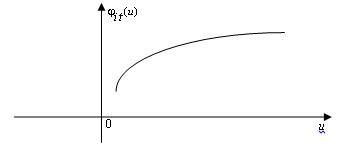
\includegraphics[scale=1]{pictures/picturefile_7_2}}
\caption{Зависимость стоимости перевозки от количества\\перевезенного груза}
\label{picture_7_2}
\end{figure}
Для составления плана нам достаточно выбрать числа $u_1(t), u_2(t)$ при $\it t=1,2,...,N$. При этом по смыслу задачи
\numberwithin{equation}{section}\begin{equation}\label{equation_7_8}
 u_1(t)\ge 0,u_2 \ge 0, u_1(t)+u_2(t) \le b_t при t = 1,2,...,N.
\end{equation}
\indentИными словами, "управляющая точка"$\vec{u}(t)=(u_1(t);u_2(t))$ должна находиться в треугольнике. Поскольку необходимо выполнить условия
 \numberwithin{equation}{section}\begin{equation*}
u_1(t) \le a_1,  u_2(t) \le a_2,
\end{equation*}
 то множество $\it U_t$ может быть пятиугольником Рис. \ref{picture_7_3}.\\
\indentСостояние складов (состояние объекта) при таком поэтапном распределении будем характеризовать величинами:\\
\indent x$_1$(t) — количество сырья, вывозимого с первого склада на первые $\it t$  заводов%%%%%%%%%%%%%%%%%%
\indent x$_2$(t) — количество сырья, вывозимого со второго склада на первые  $\it t$  заводов.\\
\indentЯсно, что
\numberwithin{equation}{section}\begin{equation}{
\begin{cases}\label{equation_7_9}
  x_1(t) = x_1(t-1)+u_1(t),\\
  x_2(t) = x_2(t-1)+u_2(t)
\end{cases}}
\end{equation}
где $\it t=1, 2,..., N.$\\
\begin{figure}[h]
\center{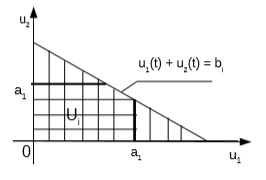
\includegraphics[scale=1]{pictures/picturefile_7_3}}
\caption{Область допустимых управлений нелинейной\\
транспортной задачи}
\label{picture_7_3}
\end{figure}
Равенства $\it (7.9)$ представляют собой уравнения состояния. Для удобства мы будем считать, что
 \numberwithin{equation}{section}\begin{equation}	\label{equation_7_10}
x_1(0)=x_2(0)=0
\end{equation}
\indentТак как запас равен спросу, то после вывоза сырья на все N  заводов склады должны остаться пустыми, т.е.
 \numberwithin{equation}{section}\begin{equation}\label{equation_7_11}
x_1(N)=a_1;x_2(N)=a_2
\end{equation}
\indentКритерием эффективности плана здесь является стоимость всех перевозок:
 \numberwithin{equation}{section}\begin{equation*}
I=\sum_{k=1}^N[\varphi_{1t}(u_1(t)+\varphi_{2t}(u_2(t))+\varphi_{3t}(b_t-u_1(t)-u_2(t))].
\end{equation*}
\indentТаким образом, транспортная задача приобретает следующую формулировку: для управляемого объекта (\ref{equation_7_9}) найти такое допустимое управление $\it u_1(t), u_2(t)$  (удовлетворяющее условию (\ref{equation_7_8})), чтобы для соответствующей траектории $x_1(t), x_2(t) (t=1,2,...,N)$ с начальным условием (\ref{equation_7_10}) удовлетворялось конечное условие (\ref{equation_7_11}) и при этом функционал $\it I$ принимал наименьшее возможное значение. Очевидно, что это частный случай задачи с подвижными концами, в которой множества $\it M_0$  и  $\it M_1$ состоят из одной точки каждое.\\
\indent{\it\bfseries 2. Задача о распределении ресурсов.} Мы рассмотрим наиболее простой вариант этой задачи. В нашем распоряжении имеется какой-то запас средств (ресурсов) в количестве $\it К$ единиц. Эти средства нужно распределить между предприятиями  П$_1$, П$_2$, ..., П$_N$. Каждое предприятие $\it П_t$  при вложении в него средств и приносит доход, зависящий от$\it u$, т.е. представляющий собой функцию  $\varphi_t(u)$, которая считается известной. Функции  $\varphi_t(u) (t=1,2,...,N)$ являются неубывающими. Задача заключается в распределении средств между предприятиями с целью получения максимального суммарного дохода. Хотя в такой постановке задача не содержит упоминания о времени, можно все же операцию распределения  средств между  предприятиями мысленно  развернуть в какой-то последовательности, считая за первый шаг вложение средств в предприятие П$_1$, за второй — в П$_2$ и т.д. Управляемым объектом здесь являются средства, а состояние объекта определяется параметром $\it x(t)$ — количеством средств, которые остаются после вложения в t-е предприятие. Управляющим параметром здесь является  $\it u(t)$ — количество средств, вложенных в предприятие П$_t$. Очевидно, что
 \numberwithin{equation}{section}\begin{equation*}
x(t)=x(t-1)-u(t), (t=1,2,...,N).
\end{equation*}
\indentЭти равенства представляют собой уравнения состояния. Управление по своему смыслу неотрицательно и не больше общей суммы наличных средств:
 \numberwithin{equation}{section}\begin{equation*}
u(t) \ge 0, u(t)  \le x(t-1)
\end{equation*}
Последние неравенства определяют множество $\it U_t(x(t-1))$  допустимости управления.Задача наша заключается в нахождении оптимального управления $\it u(1),u(2),...,u(N)$, для которого суммарный доход максимален:
\numberwithin{equation}{section}\begin{equation*}
I = \sum_{k=1}^N \varphi_t(u(t)) \rightarrow max
\end{equation*}
\indent При этом в начальный момент времени $\it x(0)=K$, кроме того,  $\it x(N)=0$. Последнее условие означает, что все средства распределяются.\\
\indent{\it\bfseries 3. Принцип оптимальности Беллмана.} Решение задач оптимального управления с дискретным временем основано на особом принципе, который называют принципом оптимальности. Метод решения этих задач называется методом динамического
программирования. Сам принцип оптимальности очень прост. Его можно пояснить следующим образом. \\
\indentКритерий оптимальности или целевой функционал  (\ref{equation_7_7}) является суммой слагаемых, каждое из которых зависит от состояния объекта в начале $\it t$-го шага и от управления, выбираемого на этом шаге процесса. Можно пытаться так выбрать управление, чтобы оптимизировать именно это  $\it t$-е слагаемое. Однако, уже выбрав управление, мы изменим состояние объекта и это, может быть, не позволит нам в будущем получить еще больший выигрыш на других слагаемых. Таким образом, шаговое управление должно выбираться дальновидно, с учетом всех его последствий в будущем. Значит, планируя многошаговую операцию, надо выбирать управление с учетом всех его будущих последствий на еще предстоящих шагах. Однако среди всех шагов есть один, который можно планировать без оглядки на будущее, чтобы он сам, как таковой, принес наибольшую выгоду. Это последний шаг. И если управление уже найдено, и в нем перед последним шагом объект находится в состоянии $\vec{x}(N-1)$ , то управление $\vec{u}(N)$ должно быть точкой максимума функции
\numberwithin{equation}{section}\begin{equation*}
f_0(N,\vec{x}(N-1),\vec{u}(N)).
\end{equation*}
\indentПравда, найти это управление нельзя, поскольку нам неизвестно состояние $\vec{x}(N-1)$ объекта перед последним шагом. Аналогично этому в оптимальном управлении перед  $\it T$-м шагом, когда объект находится в состоянии $\vec{x}(T-1)$, управления $\vec{u}(T), \vec{u}(T+1),...,\vec{u}(N),$ должны обеспечивать максимум функции
\numberwithin{equation}{section}\begin{equation}\label{equation_7_12}
I(T)=\sum_{t=T}^N f_0(t,\vec{x}(t-1), \vec{u}(t)).
\end{equation}\\
\indentТеперь можно сформулировать сам принцип.\\\\
\indent\begin{bfseries}Принцип оптимальности.\end{bfseries} \begin{it}Оптимальное управление обладает тем свойством, что каково бы ни было начальное состояние и начальное управление, последующее управление должно быть оптимальным по отношению к состоянию, получающемуся в результате действия начального управления.\end{it}\\\indentИспользование этого принципа гарантирует, что управление, выбранное на любом шаге, является не локально лучшим, а лучшим с точки зрения  процесса в целом. \\
\indentТеперь изложим в общих чертах сам метод динамического программирования. Рассматривается задача с заданным  . Уже
отмечалось, что управление на последнем шаге $\vec{u}(N)$ должно быть точкой максимума функции
\numberwithin{equation}{section}\begin{equation*}
f_0(N,\vec{x}(N-1),\vec{u}(N)).
\end{equation*}
\indentЭтот максимум определить нельзя, т.к. нам неизвестно состояние $\vec{x}(N-1)$  после $\it N-1$-го шага. Предположим, что мы можем находить максимум функции $f_0(N,\vec{x},\vec{u})$  по переменным $\vec{u}$ при любых допустимых значениях $\vec{x}$. Естественно, что точка максимума $\vec{u}$ может зависеть от значений ${x_1,x_2,...,x_N}=\vec{x}$ , т.е. $\vec{u}_{max}=\vec{u}_N(\vec{x}) = {u_{1N}(\vec{x}, u_{2N})(\vec{x}),...,u_{rN}(\vec{x})}$. Будем считать функцию $\vec{u}_{N}(\vec{x})$ определённой. При её нахождении, разумеется, учитываются ограничения на $\vec{u}(\vec{u} \in U_N(\vec{x})$  Если подставить вместо $\vec{u}$ функцию $\vec{u}(\vec{x})$ в выражение для $f_0(N,\vec{x},\vec{u})$ , то мы получим некоторую функцию \numberwithin{equation}{section}\begin{equation*}
\omega_N (\vec{x})=f_0(N,\vec{x},\vec{u}_N(\vec{x}))
\end{equation*}
\indentРассмотрим теперь $(N-1)$-й шаг. В его начале объект находится в состоянии $\vec{x}(N-2)$ , которое нам неизвестно. При этом,$x_i(N-1)=f_i(N-1, \vec{x}(N-2),\vec{u}(N-1)$  . Согласно принципу максимума $\vec{u}(N-1)$ должна быть точкой максимума функции
 \numberwithin{equation}{section}\begin{equation*}
f_0(N-1, \vec{x}(N-2),\vec{u}(N-1)) + \omega_N(\vec{f}(N-1,\vec{x}(N-2),\vec{u}(N-1)))
\end{equation*}
\indentЭтот максимум определить нет возможности, т.к. состояние $\vec{x}(N-2)$ нам неизвестно. Пусть  нам удается найти максимум функции
 \numberwithin{equation}{section}\begin{equation}\label{equation_7_13}
f_0(N-1, \vec{x},\vec{u}) + \omega_N(\vec{f}(N-1,\vec{x},\vec{u}))
\end{equation}
который в общем случае зависит от $\vec{x}$. Обозначим его через $\vec{u}_{N-1}(\vec{x})$ и, подставляя в выражение (13), получим некоторую функцию $\omega_{N-1}(\vec{x})$ . Продолжая рассматривать шаги с меньшими номерами, мы на $k$-ом шаге находим функцию
 \numberwithin{equation}{section}\begin{equation*}
\omega_{k-1}(\vec{x})=\max_{\vec{u}\in U_{r-1}(\vec{x})} (f_0(k-1, \vec{x},\vec{u})-\omega_{k}(\vec{f}(k-1,\vec{x},\vec{u}))
\end{equation*}
\indentПоследнее уравнение называется функциональным уравнением Беллмана. С помощью этого уравнения мы рекуррентно находим функции
 \numberwithin{equation}{section}\begin{equation*}
 \omega_{N}(\vec{x}), \omega_{N-1}(\vec{x}),...,\omega_{1}(\vec{x})
\end{equation*}
и также точки максимума
 \numberwithin{equation}{section}\begin{equation*}
 \vec{u}_N(\vec{x}),  \vec{u}_{N-1}(\vec{x}),...,\vec{u}_1(\vec{x}).
\end{equation*}
\indent Эти точки максимума позволяют определить оптимальное управление. Действительно, нам известно начальное состояние $\vec{x}(0)$.\\\indent Поэтому управление на первом шаге есть
 \numberwithin{equation}{section}\begin{equation*}
 \vec{u}(1) =  \vec{u}_1(\vec{x}(0)).
\end{equation*}
\indentЗная это управление, мы находим состояние в начале второго шага   с помощью уравнений состояния. Затем находим управление на втором шаге:
 \numberwithin{equation}{section}\begin{equation*}
 \vec{u}(2) =  \vec{u}_2(\vec{x}(1)).
\end{equation*}
\indent Таким образом, определяется оптимальное управление шага $t$:
 \numberwithin{equation}{section}\begin{equation*}
 \vec{u}(t) =  \vec{u}_t(\vec{x}(t-1)).
\end{equation*}
\indent Соответствующая траектория находится с помощью уравнений состояния параллельно с нахождением оптимального управления.\\
\indent В процессе оптимизации управления методом динамического программирования многошаговый процесс “проходится” дважды. Первый раз — от конца к началу, в результате чего находятся условные оптимальные управления $\vec{u}_t(\vec{x})$  и условные оптимальные выигрыши $\omega_k(\vec{x})$  за оставшийся “хвост” процесса. Второй раз процесс “проходится” от начала к концу, когда нам остается только “прочитать” уже готовые рекомендации и найти безусловное оптимальное управление $\vec{u}(t)$ состоящее из оптимальных шаговых управлений $\vec{u}(1),\vec{u}(2),...,\vec{u}(N)$
Первый этап — этап условной оптимизации — несравненно сложнее и длительнее второго. Второй этап почти не требует дополнительных вычислений.
\subsection{Пример решения задач динамического программирования}
\indent\begin{bfseries} Пример~7.1.~\end{bfseries}
Пользуясь~методом~динамического программирования, решим конкретную задачу распределения ресурсов, размер которых К=200 млн.руб., между четырьмя предприятиями П1, П2, П3, П4 (N=4). Функции дохода на каждом из четырех предприятий задаются равенствами:

 \numberwithin{equation}{section}\begin{equation*}
f_1(u) = 0,4u;
\end{equation*}
 \numberwithin{equation}{section}\begin{equation*}
f_2(u) = 0,6u;
\end{equation*}
 \numberwithin{equation}{section}\begin{equation*}
f_3(u) = 0,8u;
\end{equation*}
 \numberwithin{equation}{section}\begin{equation*}
f_4(u) = 0,7u;
\end{equation*}
\indent Таким образом, функции дохода считаются линейными, а общий целевой функционал имеет вид
 \numberwithin{equation}{section}\begin{equation*}
I = 0,4u(1)+0,6u(2)+0,8(3)+0,7u(4).
\end{equation*}
\indent Управление u(t) (t=1,2,3,4) нужно выбрать так, чтобы максимизировать $I$. Уравнения состояния здесь имеют вид
 \numberwithin{equation}{section}\begin{equation*}
x(t) = x(t-1)-u(t), t = 1,2,3,4.
\end{equation*}
\indent Управления выбираются из условий
 \numberwithin{equation}{section}\begin{equation*}
u(t) \ge 0, u(t) \le x(t-1)
\end{equation*}
\indent Кроме того, мы считаем, что  x(0) = K, x(4) = 0.
\\\indent Согласно общей схеме на последнем шаге мы максимизируем функцию $f_4(u)$ на отрезке $0\le u\le x(3)$ Очевидно максимум этой функции будет достигаться в точке $x(3)$ Таким образом, мы имеем
 \numberwithin{equation}{section}\begin{equation*}
\omega(x) = 0,7(x); u_4(x) = x.
\end{equation*}
\indent Рассмотрим теперь третий шаг. В его начале состояние есть $x(2)$, причем $x(3)=x(2)-u(3)$. Поэтому на третьем шаге мы должны максимизировать функцию
 \numberwithin{equation}{section}\begin{equation*}
0,8u(3)+0,7(x(2)-u(3))
\end{equation*}
на отрезке $0 \le u(3) \le x(2)$ Следовательно
 \numberwithin{equation}{section}\begin{equation*}
\omega_3(x) = \max_{0 \le u \le x}(0,1u+0,7x)=0,8x;u_3(x)=x.
\end{equation*}
\indent На втором шаге x(2)=x(1)-u(2), и максимизируется функция
 \numberwithin{equation}{section}\begin{equation*}
0,6u(2)+0,8(x(1)-u(2)),
\end{equation*}
то есть
 \numberwithin{equation}{section}\begin{equation*}
\omega_2(x) = \max_{0 \le u \le x}(0,8x-0,2u)=0,8x;u_2(x)=0.
\end{equation*}
\indent Наконец, на первом шаге  $x(1)=x(0)-u(1)$, и максимизируется функция
 \numberwithin{equation}{section}\begin{equation*}
0,4u(1)+0,8(x(0)-u(1));
\end{equation*}
\numberwithin{equation}{section}\begin{equation*}
\omega_1(x) = \max_{0 \le u \le x}(0,8x-0,4u)=0,8x;u_1(x)=0.
\end{equation*}
\indent Поскольку $x(0)=200$, то мы получим
 \numberwithin{equation}{section}\begin{equation*}
u(1)=u_1(200)=0;\omega_1(200)=160(=0,8*200);
\end{equation*}
 \numberwithin{equation}{section}\begin{equation*}
x(1)=200-0=200.
\end{equation*}
 \numberwithin{equation}{section}\begin{equation*}
u(2)=u_2(x(1))=u_2(200)=0;\omega_2(200)=160;
\end{equation*}
 \numberwithin{equation}{section}\begin{equation*}
x(2)=200-0=200.
\end{equation*}
 \numberwithin{equation}{section}\begin{equation*}
u(3)=u_3(x(2))=u_3(200)=200;\omega_3(200)=0;
\end{equation*}
 \numberwithin{equation}{section}\begin{equation*}
x(3)=200-200=0.
\end{equation*}
\numberwithin{equation}{section}\begin{equation*}
u(4)=u_4(x(3))=u_4(0)=0,7*0=0;\omega_4(0)=0,7*0=0;
\end{equation*}
 \numberwithin{equation}{section}\begin{equation*}
x(2)=200-0=200.
\end{equation*}
\indent Таким образом, мы имеем следующие управления:
 \numberwithin{equation}{section}\begin{equation*}
u(1)=0; u(2) = 0; u(3)=200; u(4)=0.
\end{equation*}
\indent Общий доход при этом составит $\omega$1(200) = 160 млн. руб.\\
\indent Этот результат, однако, можно было бы предвидеть заранее, поскольку третье предприятие имеет наивысший коэффициент прибыли на вложенный рубль и выгоднее всего вкладывать все средства именно в это предприятие.
\\
\indent \begin{bfseries}Пример 7.2.\end{bfseries} Решим~теперь задачу~об~оптимальных мясозаготовках. В начале периода управления на ферме имелось 1200 голов скота. Период управления 4 года. Минимальные ежегодные мясозаготовки составляют 150 голов. После периода управления численность скота на ферме не должна быть меньше 800 голов. Численность скота, оставляемого на ферме для воспроизводства, в следующем году увеличивается в 1,4 раза. Доход от продажи скота выражается функцией, представленной на Рис. \ref{picture_7_4}.
\begin{figure}[h]
\center{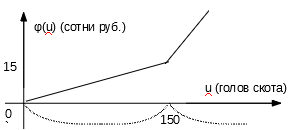
\includegraphics[scale=1]{pictures/picturefile_7_4}}
\caption{Функция $\varphi$(u) примера 7.2}
\label{picture_7_4}
\end{figure}
\indent Введем обозначения:
$x(t)$ — количество скота, оставленного на ферме к концу $t$-го года;
$u(t)$ — количество скота, проданное в $t$-ом году.
\indent Имеем уравнение состояния:
 \numberwithin{equation}{section}\begin{equation*}
x(t)=1,4x(t-1)-u(t), t=1,2,3,4.
\end{equation*}
\indent Требуется выбрать управление, чтобы максимизировать
\numberwithin{equation}{section}\begin{equation*}
I = \varphi(u(1))+\varphi(u(2))+\varphi(u(3))+\varphi(u(4)).
\end{equation*}
%%%%%%%%%%%%%%%%%%%%%%%%%%%%%%%%%%%%%%%%%%%%%%%%%%%%%%%%%%%%%%%%%%
\indent При этом 150$\le$u(t)$\le$1,4x(t-1) и x(0)=1200; x(4)$\ge$800. Последние неравенства означают, что  u(4) $\le$ 1,4x(3) - 800. \\
\indent Начинаем оптимизацию с четвертого шага. Нужно определить максимум функции
\numberwithin{equation}{section}\begin{equation*}
\varphi(u(4))  = u-135 \:\text{при}\:150 \le u(4) \le 1,4x(3)-800
\end{equation*}
\indent Поскольку функция $\varphi$ монотонно растет, то $u_4(x)=1,4x-800$,
 \numberwithin{equation}{section}\begin{equation*}
\omega_4(x)  =  1,4x - 800 - 135 = 1,4x - 935.
\end{equation*}
\indent На третьем шаге максимизируется функция  (x(3) = 1,4x(2) – u(3)):
 \numberwithin{equation}{section}\begin{equation*}
\varphi(u(3)) + \omega_4(1,4x(2)-u(3))\:при\:150 \le u(3) \le 1,4x(2),
\end{equation*}
\indent  то есть нужно определить
 \numberwithin{equation}{section}\begin{equation*}
\omega_3(x)= \max_{150\le u \le 1,4x}(u-135+1,4(1,4x-u-935))=
\end{equation*}
 \numberwithin{equation}{section}\begin{equation*}
\max_{150\le u \le 1,4x}(1,96-0,44u-1070)=1,96x-1130;
\end{equation*}
 \numberwithin{equation}{section}\begin{equation*}
u_3(x)=150.
\end{equation*}
\indent На втором шаге максимизируется функция
 \numberwithin{equation}{section}\begin{equation*}
\varphi(u(2))+\omega_3(1,4x(1)-u(2)) \:\text{при условиях}\:150\le u(2) \le 1,4x(1).
\end{equation*}
 \numberwithin{equation}{section}\begin{equation*}
\omega_1(x) = \max_{150 \le u \le 1,4x}(u-135+1,96(1,4x-u)-1130)
\end{equation*}
 \numberwithin{equation}{section}\begin{equation*}
=\max_{150 \le u \le 1,4x}(2,704x-0,96u-1265)=2,704-1409
\end{equation*}
 \numberwithin{equation}{section}\begin{equation*}
u_2(x)=150.
\end{equation*}
\indent На первом шаге максимизируется функция
 \numberwithin{equation}{section}\begin{equation*}
\varphi(u(1))+\omega_2(1,4x(0)-u(1)) \:\text{при условиях}\:150\le u(1) \le 1,4x(0).
\end{equation*}
 \numberwithin{equation}{section}\begin{equation*}
\omega_1(x) = \max_{150 \le u \le 1,4x}(u-135+2,704(1,4x-u)-1409)
\end{equation*}
 \numberwithin{equation}{section}\begin{equation*}
=\max_{150 \le u \le 1,4x}(3,7856x-0,704u-1544)=
\end{equation*}
 \numberwithin{equation}{section}\begin{equation*}
=3,7856x-1649,6;
\end{equation*}
 \numberwithin{equation}{section}\begin{equation*}
u_1(x)=150.
\end{equation*}
\indent Этап условной оптимизации закончен. Оптимальный выигрыш за четыре года составит
 \numberwithin{equation}{section}\begin{equation*}
\omega_1(x(0))=\omega_1(1200)=4542,72-1649,6=2893,12;
\end{equation*}
\numberwithin{equation}{section}\begin{equation*}
u(1)=u_1(1200)=150;
\end{equation*}
\numberwithin{equation}{section}\begin{equation*}
x(1)=1,4x(0)-u(1)=1,4*1200-150=1530;
\end{equation*}
 \numberwithin{equation}{section}\begin{equation*}
u(2)=u_2(1530)=150;
\end{equation*}
 \numberwithin{equation}{section}\begin{equation*}\setlength\parsep{-20pt}
x(2)=1,4x(1)-u(2)=1,4*1530-150=1992;
\end{equation*}
 \numberwithin{equation}{section}\begin{equation*}
u(3)=u_3(1992)=150;
\end{equation*}
 \numberwithin{equation}{section}\begin{equation*}
x(3)=1,4x(2)-u(3)=1,4*1992-150=2788,8-150=2638,8;
\end{equation*}
 \numberwithin{equation}{section}\begin{equation*}
u(4)=u_4(2638,8)=1,4*2638,8-800=2894,32;
\end{equation*}
\numberwithin
{equation}{section}\begin{equation*}x(4) = 1,4x(3)-u(4) = 800.\end{equation*}
\indentТаким образом, оптимальная стратегия в данном случае заключается в том, чтобы продавать в первые три года минимальное количество скота (150 голов), а в последнем году продать весь скот, оставив на ферме лишь 800 голов.

\indent\textbf{Пример 7.3.} Попытаемся теперь решить ту же задачу с иной функцией дохода $\varphi(u)$. Пусть эта функция имеет вид Рис. \ref{picture_7_5}\\
\[
\varphi(u) =
    \begin{cases}
        2u,u\leq300 \\
        0,5u+450,u>300.
    \end{cases}
\]
Все остальные условия предыдущей задачи остаются прежними. \\
\indentНа четвертом шаге
\[
\omega_4 =\underset{150\leq u\leq1,4(x)-800}{max}
    \begin{cases}
        2(1,4x-800)1,4x-800\leq300 \\
        0,5(4x-800)+450,1,4x-800>300.
    \end{cases}
\]
\begin{figure}[h]
\center{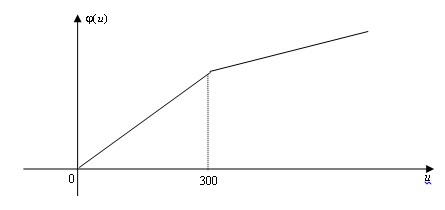
\includegraphics[scale=1]{pictures/picturefile_7_5}}
\caption{функция $\varphi(u)$ примера 7.3 }
\label{picture_7_5}
\end{figure}
\[
\omega_4 =
    \begin{cases}
        2,8x-1600,x\leq\frac{5500}7 ;\\
        0,7x-50,x>\frac{5500}7 ;
    \end{cases}
\]
\begin{center}$u4(x) = 1,4x – 800$\end{center}
На третьем шаге $(x(3) = 1,4x(2)-u(3)):$\numberwithin
{equation}{section}\begin{equation*}\omega_3(x)=\underset{150\leq u\leq1,4(x)}{\mathrm{max}}\varphi(u)+\omega_4(1,4x-u)).\end{equation*}

\indentВычисление функции $\omega_3$(x) встречает большие трудности и требует большой изобретательности. Нахождение функций  $\omega_2$(x) и  $\omega_1$(x)
%newpage
встречает еще большие трудности. Таким образом, аналитическое решение задач динамического программирования часто приводит к сложным задачам на глобальный экстремум для функций, зависящих от параметра. Преодолеть эти трудности часто удается с помощью численной реализации алгоритма динамического программирования на ЭВМ.\\
\indentПри численной реализации управляющим параметрам придают лишь дискретное множество значений, которые, например, кратны некоторым величинам. В одних задачах это новое условие является естественным, в других  — вводится  искусственно. При этом решение, полученное с этим дополнительным условием, дает приближенное представление об истинном оптимальном управлении. Так, в задаче примера 3 предположение, что сдача скота на мясозаготовки может происходить партиями по 50 голов является искусственным. Однако при этом количество возможных значений параметра u будет конечным. Конечным будет и количество возможных состояний. Предположение же, что$u$ принимает значения, кратные единице, является естественным. Однако оно приводит к очень большому числу (хотя и конечному) возможных управлений и состояний. Численная реализация задачи тем проще, чем меньше возможное количество управлений и состояний нужно рассматривать на каждом шаге управления. Поэтому предположение, что u  в примере 7.3 принимает значения, кратные 50, приводит к более простой численной реализации задачи. Впрочем, проследить эту реализацию и в этом случае для нас сложно из-за большого числа возможных управлений.\\
\indent\textbf{Пример 7.4.} Рассмотрим задачу о распределении ресурсов. Исходный запас средств К=10 (условных единиц). Требуется  его оптимальным образом распределить между пятью (N=5) предприятиями. Предполагается, что вкладываются лишь целые количества средств. Функции дохода $\varphi_t$(u) заданы  в следующей таблице:
\begin{center}
\begin{tabular}[c]{|c|c|c|c|c|c|}
\hline
$\mspace{15mu}u\mspace{15mu}$&$\varphi_1$(u)&$\varphi_2$(u)&$\varphi_3$(u)&$\varphi_4$(u)&$\varphi_5$(u) \\
\hline
1&0,5&0,1&0,6&0,3&1,0\\  [0.02cm]
\hline
2&1,0&0,5&1,1&0,6&1,2\\ [0.02cm]
\hline
3&1,4&1,2&1,2&1,3&1,3\\ [0.02cm]
\hline
4&2,0&1,8&1,4&1,4&1,3\\ [0.02cm]
\hline
5&2,5&2,5&1,6&1,5&1,3\\ [0.02cm]
\hline
6&2,8&2,9&1,7&1,5&1,3\\ [0.02cm]
\hline
7&3,0&3,5&1,8&1,5&1,3\\ [0.02cm]
\hline
\end{tabular}
\end{center}
%newpage

\indentВ каждом столбце, начиная с какой-то суммы вложений, доходы перестают возрастать (остаются постоянными). Это связано с тем, что каждое предприятие способно "освоить" лишь ограниченное количество средств. Число возможных значений u на первом шаге равно 11 (с учетом значения  $u$=0). Поскольку функция $\varphi_t$(u) стабилизируется при t$\geq$7, мы не приводим еще трех  строк этой таблицы. Напомним, что уравнение состояния здесь имеет вид\numberwithin
{equation}{section}\begin{equation*}x(t)=x(t-1)-u(t),t=1,2,3,4,5\end{equation*}
\indentгде $x(t)$ — количество еще не распределенных средств;$u(t)$ — количество средств, выделяемых предприятию с номером $t$,\numberwithin
{equation}{section}\begin{equation*}0\leq u(t)\leq x(t-1),   t = 1, 2, 3, 4, 5.\end{equation*}
\indentКроме того,$u(t)$ при каждом $t$ может принимать целые значения.\numberwithin
{equation}{section}\begin{equation*}x(0) = 10,  x(5) = 0.\end{equation*}
\indentМы должны максимизировать функцию  $I=\sum\limits_{t=1}^5\varphi_t(u(t)).$\\
\indentПри $t$=5 мы находим  $\omega_5(x)=\underset{0\leq u\leq x}{\mathrm{max}}\varphi_5(u)$\\
\indentПоскольку функция $\varphi_5$(x) не убывающая, то  $\omega_5(x)=\varphi_5(x), u_5(x)=x$.\\
\indentРезультаты условной оптимизации заносим в следующую таблицу:
\begin{center}
\begin{tabular}[t]{|c|c|c|c|c|c|c|c|c|c|c|c|}
\hline
 &\multicolumn{2}{|c|}{$t$=5}&\multicolumn{2}{|c|}{$t$=4}&\multicolumn{2}{|c|}{$t$=3}&\multicolumn{2}{|c|}{$t$=2}&\multicolumn{2}{|c|}{$t$=1}\\
\hline
$x$ & $u_5$ & $\omega_5$ & $u_4$ & $\omega_4 $& $u_3$ & $\omega_5$ & $u_2$ & $\omega_2 $ & $u_1$ & $\varpi_1$ \\  [0.1cm]
\hline
1&\boxed{1}& 1,0&\boxed{0}& 1,0&0&1,0&0&1,0& & \\ [0.05cm]
\hline
2&2&1,2&1&	1,3&1&1,6&0&1,6& & \\ [0.05cm]
\hline
3&3&1,3&2&1,6&2&2,1&0&2,1& & \\[0.05cm]
\hline
4&4&1,3&3&	2,3&2	&2,4&	0&2,4& & \\[0.05cm]
\hline
5&5&1,3&3&	2,5&1&2,9&0&2,9& & \\[0.05cm]
\hline
6&6&1,3&4&	2,6&2&3,4&5&3,5& & \\[0.05cm]
\hline
7&7&1,3&4&	2,7&2&3,6&5&4,1& & \\[0.05cm]
\hline
8&8&1,3&5&	2,8&4&3,7&\boxed{5}&4,6& & \\[0.05cm]
\hline
9&9&1,3&6&	2,8&5&3,9&7&5,1& & \\[0.05cm]
\hline
10&10&1,3&7&2,8&5&4,1&7&5,6&\boxed{2} &\boxed{5, 6}\\[0.05cm]
\hline
\end{tabular}
\end{center}
%newpage
\indentЗаполняя эту таблицу при $t = 4$, мы находим\numberwithin
{equation}{section}
\begin{equation*} \omega_4(x)=\underset{0\leq u\leq x}{\mathrm{max}}(\varphi_4(u)+\omega_4(x-u)).\end{equation*}
\indentНахождение максимума производится непосредственно при каждом $x:$\\
\begin{flushleft}
\begin{tabular}[c]{c|c|c|c|c  }
\cline{2-4}
$x=1\mspace{10mu}$&$\mspace{15mu}u\mspace{15mu}$&\multicolumn{2}{|c|}{$\mspace{20mu}\varphi_4(u)+\omega_5(1-u)\mspace{18mu}$}& \\ [0.07cm]
\cline{2-4}
 &0&$\mspace{40mu}0+1,0\mspace{30mu}$&\boxed{1,0}&$\mspace{32mu}\omega_4$(1)=1,0\\[0.07cm]
\cline{2-4}
 &1&$0,3+0$&0,3&$\mspace{18mu}u_4$(1)=0\\[0.07cm]
\cline{2-4}
\end{tabular}
\end{flushleft}

\begin{flushleft}
\begin{tabular}[c]{c|c|c|c|c  }
\cline{2-4}
$x=2\mspace{10mu}$&$\mspace{15mu}u\mspace{15mu}$&\multicolumn{2}{|c|}{$\mspace{20mu}\varphi_4(u)+\omega_5(2-u)\mspace{18mu}$}& \\[0.07cm]
\cline{2-4}
 &0&$\mspace{40mu}0+1,2\mspace{30mu}$&1,2&$\mspace{32mu}\omega_4$(2)=1,3\\[0.07cm]
\cline{2-4}
 &1&0,3+1,0&$\boxed{1,3}$&$\mspace{18mu}u_4$(2)=1\\[0.07cm]
\cline{2-4}
 &2&$0,6+0$&0,6\\[0.07cm]
\cline{2-4}
\end{tabular}
\end{flushleft}

\begin{flushleft}
\begin{tabular}[c]{c|c|c|c|c  }
\cline{2-4}
$x=3\mspace{10mu}$&$\mspace{15mu}u\mspace{15mu}$&\multicolumn{2}{|c|}{$\mspace{20mu}\varphi_4(u)+\omega_5(3-u)\mspace{18mu}$}& \\[0.07cm]
\cline{2-4}
 &0&$\mspace{40mu}0+1,3\mspace{30mu}$&1,3&$\mspace{32mu}\omega_4$(3)=1,6\\[0.07cm]
\cline{2-4}
 &1&0,3+1,2&$1,5$&$\mspace{18mu}u_4$(3)=2\\[0.07cm]
\cline{2-4}
 &2&$0,6+1,0$&$\boxed{1,6}$\\[0.07cm]
\cline{2-4}
 &3&$1,3+0$&1,3\\[0.07cm]
\cline{2-4}
\end{tabular}
\end{flushleft}

\begin{flushleft}
\begin{tabular}[c]{c|c|c|c|c  }
\cline{2-4}
$x=4\mspace{10mu}$&$\mspace{15mu}u\mspace{15mu}$&\multicolumn{2}{|c|}{$\mspace{20mu}\varphi_4(u)+\omega_5(4-u)\mspace{18mu}$}& \\[0.07cm]
\cline{2-4}
 &0&$\mspace{40mu}0+1,3\mspace{30mu}$&1,3&$\mspace{32mu}\omega_4$(4)=2,3\\[0.07cm]
\cline{2-4}
 &1&0,3+1,3&$1,6$&$\mspace{18mu}u_4$(4)=3\\[0.07cm]
\cline{2-4}
 &2&$0,6+1,2$&$1,8$\\[0.07cm]
\cline{2-4}
 &3&$1,3+1,0$&\boxed{2,3}\\[0.07cm]
\cline{2-4}
 &4&$1,4+0$&$1,4$\\[0.07cm]
\cline{2-4}
\end{tabular}
\end{flushleft}

\begin{flushleft}
\begin{tabular}[c]{c|c|c|c|c  }
\cline{2-4}
$x=5\mspace{10mu}$&$\mspace{15mu}u\mspace{15mu}$&\multicolumn{2}{|c|}{$\mspace{20mu}\varphi_4(u)+\omega_5(5-u)\mspace{18mu}$}& \\[0.07cm]
\cline{2-4}
 &0&$\mspace{40mu}0+1,3\mspace{30mu}$&1,3&$\mspace{32mu}\omega_4$(5)=2,5\\[0.07cm]
\cline{2-4}
 &1&0,3+1,3&$1,6$&$\mspace{18mu}u_4$(5)=3\\[0.07cm]
\cline{2-4}
 &2&$0,6+1,3$&$1,9$\\[0.07cm]
\cline{2-4}
 &3&$1,3+1,2$&\boxed{2,5}\\[0.07cm]
\cline{2-4}
 &4&$1,4+1,0$&$2,4$\\[0.07cm]
\cline{2-4}
 &5&$1,5+0$&$1,5$\\[0.07cm]
\cline{2-4}
\end{tabular}
\end{flushleft}
%newpage

\begin{flushleft}
\begin{tabular}[c]{c|c|c|c|c  }
\cline{2-4}
$x=6\mspace{10mu}$&$\mspace{15mu}u\mspace{15mu}$&\multicolumn{2}{|c|}{$\mspace{20mu}\varphi_4(u)+\omega_5(6-u)\mspace{18mu}$}& \\[0.07cm]
\cline{2-4}
 &0&$\mspace{40mu}0+1,3\mspace{30mu}$&1,3&$\mspace{32mu}\omega_4$(6)=2,6\\[0.07cm]
\cline{2-4}
 &1&0,3+1,3&$1,6$&$\mspace{18mu}u_4$(6)=4\\[0.07cm]
\cline{2-4}
 &2&$0,6+1,3$&$1,9$\\[0.07cm]
\cline{2-4}
 &3&$1,3+1,3$&2,6\\[0.07cm]
\cline{2-4}
 &4&$1,4+1,2$&$\boxed{2,6}$\\[0.07cm]
\cline{2-4}
 &5&$1,5+1,0$&$2,5$\\[0.07cm]
\cline{2-4}
 &6&$1,5+0$&$1,5$\\[0.07cm]
\cline{2-4}
\end{tabular}
\end{flushleft}

\begin{flushleft}
\begin{tabular}[c]{c|c|c|c|c  }
\cline{2-4}
$x=7\mspace{10mu}$&$\mspace{15mu}u\mspace{15mu}$&\multicolumn{2}{|c|}{$\mspace{20mu}\varphi_4(u)+\omega_5(7-u)\mspace{18mu}$}& \\[0.07cm]
\cline{2-4}
 &0&$\mspace{40mu}0+1,3\mspace{30mu}$&1,3&$\mspace{32mu}\omega_4$(7)=2,7\\[0.07cm]
\cline{2-4}
 &1&0,3+1,3&$1,6$&$\mspace{18mu}u_4$(7)=4\\[0.07cm]
\cline{2-4}
 &2&$0,6+1,3$&$1,9$\\[0.07cm]
\cline{2-4}
 &3&$1,3+1,3$&2,6\\[0.07cm]
\cline{2-4}
 &4&$1,4+1,3$&$\boxed{2,7}$\\[0.07cm]
\cline{2-4}
 &5&$1,5+1,2$&$2,7$\\[0.07cm]
\cline{2-4}
 &6&$1,5+1,0$&$2,5$\\[0.07cm]
\cline{2-4}
 &7&$1,5+0$&$1,5$\\[0.07cm]
\cline{2-4}
\end{tabular}
\end{flushleft}

\begin{flushleft}
\begin{tabular}[c]{c|c|c|c|c  }
\cline{2-4}
$x=8\mspace{10mu}$&$\mspace{15mu}u\mspace{15mu}$&\multicolumn{2}{|c|}{$\mspace{20mu}\varphi_4(u)+\omega_5(8-u)\mspace{18mu}$}& \\[0.07cm]
\cline{2-4}
 &0&$\mspace{40mu}0+1,3\mspace{30mu}$&1,3&$\mspace{32mu}\omega_4$(8)=2,8\\[0.07cm]
\cline{2-4}
 &1&0,3+1,3&$1,6$&$\mspace{18mu}u_4$(8)=5\\[0.07cm]
\cline{2-4}
 &2&$0,6+1,3$&$1,9$\\[0.07cm]
\cline{2-4}
 &3&$1,3+1,3$&2,6\\[0.07cm]
\cline{2-4}
 &4&$1,4+1,3$&$2,7$\\[0.07cm]
\cline{2-4}
 &5&$1,5+1,3$&$\boxed{2,8}$\\[0.07cm]
\cline{2-4}
 &6&$1,5+1,2$&$2,7$\\[0.07cm]
\cline{2-4}
 &7&$1,5+1,0$&$2,5$\\[0.07cm]
\cline{2-4}
 &8&$1,5+0$&$1,5$\\[0.07cm]
\cline{2-4}
\end{tabular}
\end{flushleft}
%newpage

\begin{flushleft}
\begin{tabular}[c]{c|c|c|c|c  }
\cline{2-4}
$x=9\mspace{10mu}$&$\mspace{15mu}u\mspace{15mu}$&\multicolumn{2}{|c|}{$\mspace{20mu}\varphi_4(u)+\omega_5(9-u)\mspace{18mu}$}& \\[0.07cm]
\cline{2-4}
 &0&$\mspace{40mu}0+1,3\mspace{30mu}$&1,3&$\mspace{32mu}\omega_4$(9)=2,8\\[0.07cm]
\cline{2-4}
 &1&0,3+1,3&$1,6$&$\mspace{18mu}u_4$(9)=6\\[0.07cm]
\cline{2-4}
 &2&$0,6+1,3$&$1,9$\\[0.07cm]
\cline{2-4}
 &3&$1,3+1,3$&2,6\\[0.07cm]
\cline{2-4}
 &4&$1,4+1,3$&$2,7$\\[0.07cm]
\cline{2-4}
 &5&$1,5+1,3$&$2,8$\\[0.07cm]
\cline{2-4}
 &6&$1,5+1,3$&$\boxed{2,8}$\\[0.07cm]
\cline{2-4}
 &7&$1,5+1,2$&$2,7$\\[0.07cm]
\cline{2-4}
 &8&$1,5+1,0$&$2,5$\\[0.07cm]
\cline{2-4}
 &9&$1,5+0$&$1,5$\\[0.07cm]
\cline{2-4}
\end{tabular}
\end{flushleft}


\begin{flushleft}
\begin{tabular}[c]{c|c|c|c|c  }
\cline{2-4}
$x=10\mspace{1mu}$&$\mspace{15mu}u\mspace{15mu}$&\multicolumn{2}{|c|}{$\mspace{20mu}\varphi_4(u)+\omega_5(10-u)\mspace{18mu}$}& \\[0.07cm]
\cline{2-4}
 &0&$\mspace{40mu}0+1,3\mspace{30mu}$&1,3&$\mspace{32mu}\omega_4$(10)=2,8\\[0.07cm]
\cline{2-4}
 &1&0,3+1,3&$1,6$&$\mspace{18mu}u_4$(10)=7\\[0.07cm]
\cline{2-4}
 &2&$0,6+1,3$&$1,9$\\[0.07cm]
\cline{2-4}
 &3&$1,3+1,3$&2,6\\[0.07cm]
\cline{2-4}
 &4&$1,4+1,3$&$2,7$\\[0.07cm]
\cline{2-4}
 &5&$1,5+1,3$&$2,8$\\[0.07cm]
\cline{2-4}
 &6&$1,5+1,3$&$2,8$\\[0.07cm]
\cline{2-4}
 &7&$1,5+1,3$&$\boxed{2,8}$\\[0.07cm]
\cline{2-4}
 &8&$1,5+1,2$&$2,7$\\[0.07cm]
\cline{2-4}
 &9&$1,5+1,0$&$2,5$\\[0.07cm]
\cline{2-4}
 &10&$1,5+0$&$1,5$\\[0.07cm]
\cline{2-4}
\end{tabular}
\end{flushleft}


\indentПри $t=3$ мы находим\numberwithin
{equation}{section}\begin{equation*}\omega_3(x)=\underset{0\leq u\leq x}{\mathrm{max}}(\varphi_3(u)+\omega_4(x-u)).\end{equation*}

\indentСоответствующие столбцы для $t=3$ заполняются аналогично с использованием столбца для $\omega_4(x)$ и столбца $\varphi_3(x)$ таблицы функций дохода. Так же мы заполняем и столбцы, отвечающие $t=2$. При этом\numberwithin
{equation}{section}\begin{equation*}\omega_2(x)=\underset{0\leq u\leq x}{\mathrm{max}}(\varphi_2(u)+\omega_4(x-u)).\end{equation*}

\indentПри заполнении столбцов для $t=1$ можно ограничиться случаем $x=10$, поскольку начальное состояние $x(0)=10, u(1)=u1(10)=2$. Максимальная прибыль здесь равна $5,6$ условных единиц. Состояние при $t=1  x(1)=x(0)-u(1)=10-2=8$. По таблице значений $u2(x)$ находим  $u2(8)=u(2)=5$. Потом $x(2)=x(1)-u(2)=8-5=3$. Далее $u(3)=u3(3)=2$, $x(3)=x(2)-u(3)=3-2=1$, $u(4)=u4(1)=0$, $x(4)=x(3)-u(4)=1-0=1$.\\
\indentТаким образом, мы имеем следующее оптимальное управление:\numberwithin
{equation}{section}\begin{equation*}u(1)=2,  u(2)=5,  u(3)=2,  u(4)=0,  u(5)=1,\end{equation*}
т.е. первому предприятию следует выделить 2 ед. средств, второму — 5 ед., третьему —2 ед., четвертому — 0 ед. и пятому — 1 ед.\\

\addcontentsline{toc}{subsection}{Контрольные вопросы и задачи для самостоятельного решения}
\subsection*{Контрольные вопросы и задачи для самостоятельного решения}
\begin{enumerate}
  \item{Что входит в описание дискретного управляемого объекта? Приведите пример дискретного управляемого объекта, определив для него переменные состояния, управляющие параметры, уравнение состояния и целевой функционал.}
  \item{В чем заключается основная задача оптимального управления дискретным управляемым объектом? Сформулируйте задачу с подвижными концами, а также задачу с ограничениями на фазовые переменные.}
  \item{Дайте содержательную и математическую формулировки нелинейной транспортной задачи.}
  \item{Сформулируйте задачу об оптимальном распределении ресурсов в виде задачи оптимального управления.}
  \item{В чем заключается принцип оптимальности Беллмана?}
  \item{Опишите метод динамического программирования?}
\end{enumerate}

\indentРешение каждой содержательной задачи состоит из двух этапов:   1) этап формализации, то есть составление оптимизационной математической  модели; 2) этап решения задачи с помощью того или иного метода. Для задач динамического программирования этап формализации требует выделения управляемой системы, переменных состояния, управляющих параметров (управлений), составления уравнений состояния и целевого функционала. Этап формализации часто вызывает значительные трудности. \\

\indent{{\small\itПо изложенным выше образцам формализовать задачи} }\textbf{7.1; 7.2.}\\
\newpage
\indent\zadanie{В склад емкостью W(м$_{}^3)$ требуется поместить $N$ различных типов оборудования. Объем одной единицы оборудования i-го типа (i=1,2,3,...,$N$) равен $\mathrm{V}_i$(м$_{}^3)$.  Стоимость единицы оборудования  i-го типа равна $\mathrm{C}_i$(руб). Определить, сколько оборудования каждого типа следует поместить в склад, чтобы общая стоимость складированного оборудования была максимальной.}
\indent\zadanie{Детали $N$ видов могут обрабатываться на двух станках. Время обработки детали $i$-го вида  (i=1,2,3,...,N) на первом станке равно $a_i$  минут, а на втором станке-$b_i$  минут. Очередность  обработки  одна  и та же: сначала деталь обрабатывается на первом станке, а затем на втором. Требуется выбрать такую последовательность обработки деталей, при которой время изготовления всех деталей будет минимальным.}\\
\indent{\itСледующие конкретные задачи решить методом динамического программирования. }
\indent\zadanie{Найти оптимальный план загрузки склада в условиях задачи 7.1 при  W=90м$_{}^3$; $N$=3; $\mathrm{v}_1$=24м$_{}^3$; $\mathrm{v}_2$= 19м$_{}^3$; $\mathrm{v}_3$=16м$_{}^3$;  $\mathrm{c}_1$=960руб; $\mathrm{c}_2$=500руб; $\mathrm{c}_3$=250руб.}
\indent\zadanie{Найти оптимальную последовательность обработки деталей в условиях задачи 7.2 при $N$=4; $a_1$=20мин; $a_2$= 35мин; $a_3$=15мин;  $a_4$=50мин; $b_1$=5мин; $b_2$=10 мин; $b_3$=20мин; $b_4$=7мин.}
\indent\zadanie{Найти оптимальное распределение средств К=700тыс.руб. между тремя предприятиями, если зависимость между капиталовложениями и приростом выпуска продукции задается следующей таблицей:}
\begin{flushleft}
\begin{tabular}{|c|c|c|c|}
\hline
{\smallОбъем }&\multicolumn{3}{|c|}{{\small Прирост выпуска продукции}}\\
{\smallкапиталовложений}&\multicolumn{3}{|c|}{{\small(тыс. руб.)}}\\
\hline
{\small(тыс. руб.)}&{\smallПредприятие 1}&{\smallПредприятие 2}&{\smallПредприятие 3}\\
\hline
0&0&0&0\\
\hline
100&30&50&40\\
\hline
200&50&80&50\\
\hline
300&90&90&110\\
\hline
400&110&150&120\\
\hline
500&170&190&180\\
\hline
600&180&210&220\\
\hline
700&210&220&240\\
\hline
\end{tabular}
\end{flushleft}
%newpage

\indentОптимальное распределение средств должно обеспечить максимальный суммарный  прирост выпуска продукции.
\indent\zadanie{Решить методом динамического программирования линейную транспортную  задачу со следующими условиями:}

\begin{center}
\begin{tabular}{|p{4em}|p{5em}|p{5em}|p{5em}|p{5em}|}
\hline
 &\multicolumn{4}{|c|}{Потребности}\\
\cline{2-5}
\raisebox{1.5ex}[0cm][0cm]{Запасы}&$\mspace{36mu}$70&$\mspace{36mu}$10&$\mspace{36mu}$20&$\mspace{36mu}$20\\
\hline
$\mspace{27mu}$50&\boxed{1}&\boxed{3}&\boxed{4}&\boxed{2}\\[0.2cm]
\hline
$\mspace{27mu}$45&\boxed{7}&\boxed{6}&\boxed{3}&\boxed{1}\\[0.2cm]
\hline
$\mspace{27mu}$25&\boxed{9}&\boxed{4}&\boxed{8}&\boxed{2}\\[0.2cm]
\hline
\end{tabular}
\end{center}
